\documentclass{article}
\usepackage{enumitem}
\usepackage{graphicx}
\usepackage[utf8]{inputenc}
\usepackage{listings, xcolor}
\usepackage[hyphens,spaces,obeyspaces]{url}
\usepackage{placeins}




\graphicspath{ {./pictures/} }

\author{Kenneth Hansen- cph-kh415@cphbusiness.dk
    \and Martin Høigaard Cupello - cph-mr221@cphbusiness.dk}

\title{Supervised Classifiers Comparison} 

\begin{document}
\maketitle
\thispagestyle{empty}
\tableofcontents
\clearpage

\section{Introduction}
In this paper we will compare different machine learning classifiers, and try to determine which one is the most accurate for supervised classification. We will use the popular iris dataset, to test different supervised machine learning algorithms, collect metrics, and finally test our findings against two other datasets to see if we can confirm our results and compare accuracy scores to find the best model.

\section{Supervised learning}
Supervised learning is a type of artificial intelligence and also a machine learning algorithm. The algorithm takes an input variable x and an output y, to learn how the input gets the desired output Y = f(X). This is normally done with a training dataset to produce an accurate prediction. It can be divided into two groups: Classification, where the model assigns a category based on the given input,  and regression, which is used to understand the relationship between dependent and independent variables.

In this paper, we will be using classification models to make predictions.

\subsection{KNN}
KNN (K Nearest Neighbor) tries to determine which group the data belongs to, based on proximity to the nearest neighbors.
KNN does not make any assumptions; it only uses input data which makes an educated guess of the output based on its closest neighbors.
How to choose K:
A good estimate to choose K is to take the square root of n, where n is the size of your training data. However, depending on the size of the dataset, it might not be the best.

\subsection{Gaussian Naive Bayes and Multinomial Naive Bayes}
These classifiers are called “probabilistic classifiers” and use statistics by adding the probability of each input parameter to determine which category the data is most likely to belong to. They are called “naive” since they all treat variables as independent of each other, but they use different algorithms to predict the result.
The gaussian naive bayes uses a gaussian distribution, where the probability is calculated using the standard deviation and mean for each input.
The multinomial naive bayes assumes that all distributions are multinomial, which means more than 2 input variables.


\subsection{Decision Tree}
The decision tree is a tree-like structure consisting of nodes and branches. The root node is the starting point which is the entire dataset. Then the node is split into decision nodes, based on the labels attributes.
At the end of the tree we have terminal nodes which are our labels, and the classifications which we are trying to determine. 
This is better explained by using the picture below. Assume we have a dataset consisting of animal attributes, and we are trying to determine which animal we have based on its attributes. First we ask if it has feathers, and based on this decision node we can split the tree into several branches because we know, based on this decision, if it is a bird or not. We can then work our way down the tree until we reach a terminal node with a classification.

\begin{figure}[!h]
    \centering
      \includegraphics[scale=0.4]{{animalTree}.png}
      \caption{Decision Tree}
  \end{figure}

\section{Iris Dataset}
Before we start our comparison we will explain our dataset. Our dataset is of the flower iris, and has 4 columns, sepal-length, sepal-width, petal-length and petal-width. With this information about the flower we can predict which species of flower the iris is. 
\subsection{Classifiers comparison}

\begin{figure}[!h]
  \caption{KNN classifier}
  \centering
      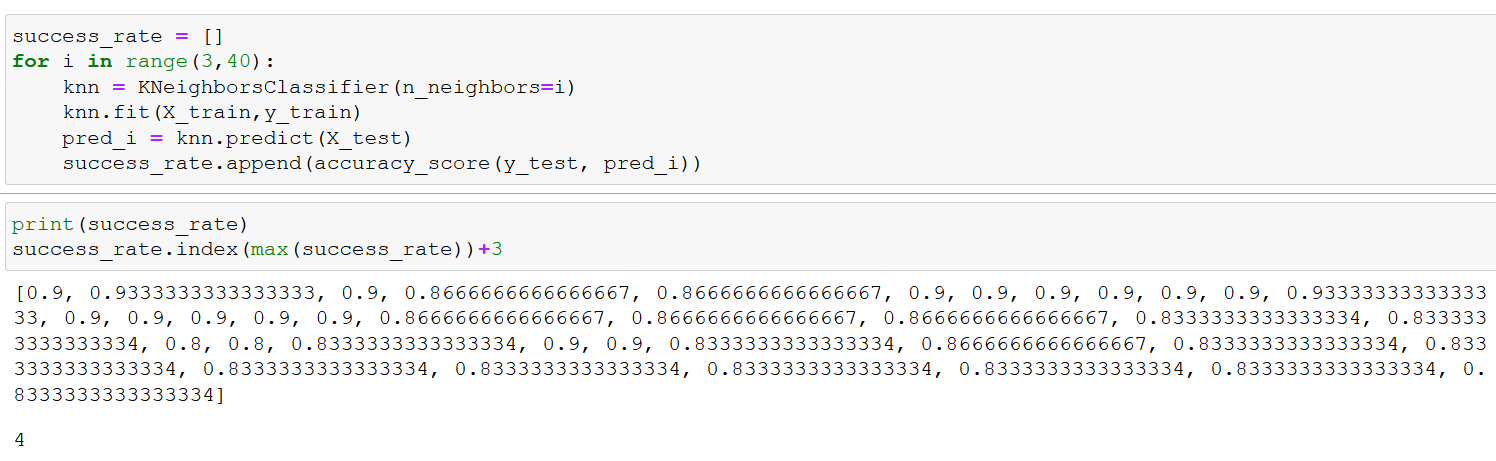
\includegraphics[width=\textwidth]{knnIris.png}
\end{figure}
\FloatBarrier

Above picture shows that 4 is actually the best value for K as it gives a higher success rate with a train/test split of 80%/20%. 



\begin{figure}[!h]
  \caption{KNN Accurracy Score}
  \centering
      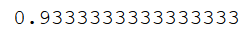
\includegraphics[scale=0.7]{successIris.png}
\end{figure}


\begin{figure}[!h]
  \centering
  \caption{Gaussian Accurracy Score}
    \includegraphics[scale=0.7]{GaussianIris.png}
\end{figure}


\begin{figure}[!h]
  \caption{Multinomial Accurracy Score}
  \centering
    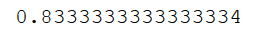
\includegraphics[scale=0.7]{multiIris.png}
\end{figure}

\begin{figure}[!h]
  \caption{Decision Tree Accurracy Score}
  \centering
    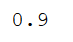
\includegraphics[scale=0.7]{treeIris.png}
\end{figure}
\FloatBarrier

\subsection{Results}
After optimizing and testing each classifier on the dataset, the results suggest that knn is the best classifier for a data set with few attributes and a size of 150 rows. To test this new hypothesis we will take a similar sized dataset and apply the same classifiers to this data. 

\section{Penguin Dataset}
We are using the penguins data set for this experiment.On this dataset we will try to classify which species a penguin is, based on a penguins features. Since the penguins dataset are about double the size of the iris dataset (a little longer actually), we first take a sample of 45\% of the full penguins dataset. This leaves us with 150 entries in the sample, close enough to say that it is similar to the length of the iris dataset.  We can now begin applying the models.
\subsection{Classifiers comparison}

\begin{figure}[!h]
  \caption{KNN Accurracy Score}
  \centering
      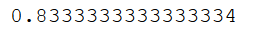
\includegraphics[scale=0.7]{knnPenguin.png}
\end{figure}


\begin{figure}[!h]
  \centering
  \caption{Gaussian Accurracy Score}
    \includegraphics[scale=0.7]{GaussianPenguin.png}
\end{figure}


\begin{figure}[!h]
  \caption{Multinomial Accurracy Score}
  \centering
    
\includegraphics[scale=0.7]{multiPenguin.png}
\end{figure}

\begin{figure}[!h]
  \caption{Decision Tree Accurracy Score}
  \centering
    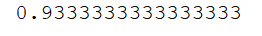
\includegraphics[scale=0.7]{treePenguin.png}
\end{figure}
\FloatBarrier

\subsection{Results}
After testing each classifier on the penguin data, we can see that our hypotheses were incorrect. We assumed that a similar sized dataset would give us the same results, but the results clearly show KNN is not the best one in this case. Gaussian Naive Bayes and Decision Tree were more accurate on the penguin dataset.
\section{Wine Quality Dataset}
Our last test will be on the wine-quality dataset. It is larger than the iris and penguins dataset combined. On this dataset we will try to classify if the wine is red or white, based on the wines physico-chemical content and its quality. Our assumption on this dataset is that since Decision Tree has performed consistently well on the two previous datasets  (93,3\% on penguins and 90\% on the iris dataset), that it will also perform well on the wine-quality dataset, even though it is larger.
\subsection{Classifiers comparison}

\begin{figure}[!h]
  \caption{KNN Accurracy Score}
  \centering
      
\includegraphics[scale=0.7]{knnWine.png}
\end{figure}


\begin{figure}[!h]
  \centering
  \caption{Gaussian Accurracy Score}
    \includegraphics[scale=0.7]{GaussianWine.png}
\end{figure}


\begin{figure}[!h]
  \caption{Multinomial Accurracy Score}
  \centering
    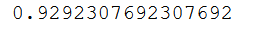
\includegraphics[scale=0.7]{multiWine.png}
\end{figure}

\begin{figure}[!h]
  \caption{Decision Tree Accurracy Score}
  \centering
    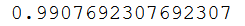
\includegraphics[scale=0.7]{treeWine.png}
\end{figure}
\FloatBarrier

\subsection{Results}
Our results on this dataset shows that the decision tree is the best classifier in our case, while Multinomial Naive Bayes continues to be the worst of them all.

\section{Results comparison}
KNN (93,3\%, 83,3\%, 94,9\%)   \hfill            $\approx$ 90,5\%  \\
Gaussian Naive Bayes (83,3\%, 93,3\%, 98\%) \hfill     $\approx$ 91,5\%  \\
Multinomial Naive Bayes (83,3\%, 80\%, 93\%) \hfill     $\approx$ 85,4\% \\
Decision Tree (90,0\%, 93,3\%, 99,1\%) \hfill         $\approx$ 94,1\% \\
\\
From our results we can see that Decision Tree performs well in most cases, though it is not the most accurate one in all cases. Worst of all in MultiNomial Naive Bayes which got the lowest score in all cases.

\section{Conclusion}
In the end we can debunk our original hypothesis that there is a best classifier. We can conclude this because given our results there was no classifier that had the highest score on all of the datasets.It is impossible to decide beforehand which one is the best. We can then conclude that to find  the best classifier for your dataset, you have to try different models and see which one provides the best result.


\section{Bibliography}
\nocite{*}
\raggedright
\bibliography{bibliographyClassifier.bib}
\bibliographystyle{plain}
 

\end{document}
